\documentclass[letterpaper,12pt]{article}
\usepackage[utf8]{inputenc}
\usepackage{booktabs}
\usepackage{tabularx}
\usepackage{makecell}
\usepackage{graphicx}
\usepackage{svg}
\usepackage{caption}
\usepackage{wrapfig}

\graphicspath{{./figs/}}
\def\svgwidth{\textwidth}



\renewcommand{\theadalign}{bl}
\renewcommand\theadfont{\bfseries}

\newcommand{\itwoc}{I\textsuperscript{2}C}


%opening
\title{Modular Electric Skateboard}
\author{Nick Fajardo, Phillip Konyeaso, Zane Weissman}

\begin{document}
\tableofcontents
\listoffigures
\listoftables

\maketitle

\begin{abstract}
The Modular Electric Skateboard (MESB) is an electric skateboard (ESB) that allows the user to mix and match components tailored to a specific user’s needs. The MESB is equipped with a TBD watt motor controlled by a handheld RC controller and capable of acheiving speeds as high as TBD. The deck, the part of the board on which the user stands while riding, can be disassembled and reassembled by hand to swap out major mechanical components of the board. The board's electrical system includes rails for mounting hot-swappable accessories.

\end{abstract}

\section{Background}
There are many means of transportation available in cities; some are more time consuming than others. Though cars are nearly ubiquitous in America, bicycles, buses, and trains remain popular alternatives. Recently, electric skateboards have filled a particular niche for some travelers. They have the advantages of decent speed (often above 20 mph) and good portability but are often held back by low range, making them ideal for short rides and trips that include trains or buses as well. Electric skateboards and similar devices can take many forms; the market is still new, but most are recognizable as a skateboard or longboard with a motor and drive train, an enclosure for batteries and electronics, and a handheld speed controller which may be wired or wireles.
\subsection{Skateboard Parts and Terminology}
Skateboarding has been around since the mid 1900s, and has changed drastically since its inception. Figures \ref{parts1} and \ref{parts2} show the different parts that make a modern complete skateboard, and the list below defines each part in detail.
\begin{figure}[!htbp]\centering
\begin{minipage}{.5\textwidth}\centering
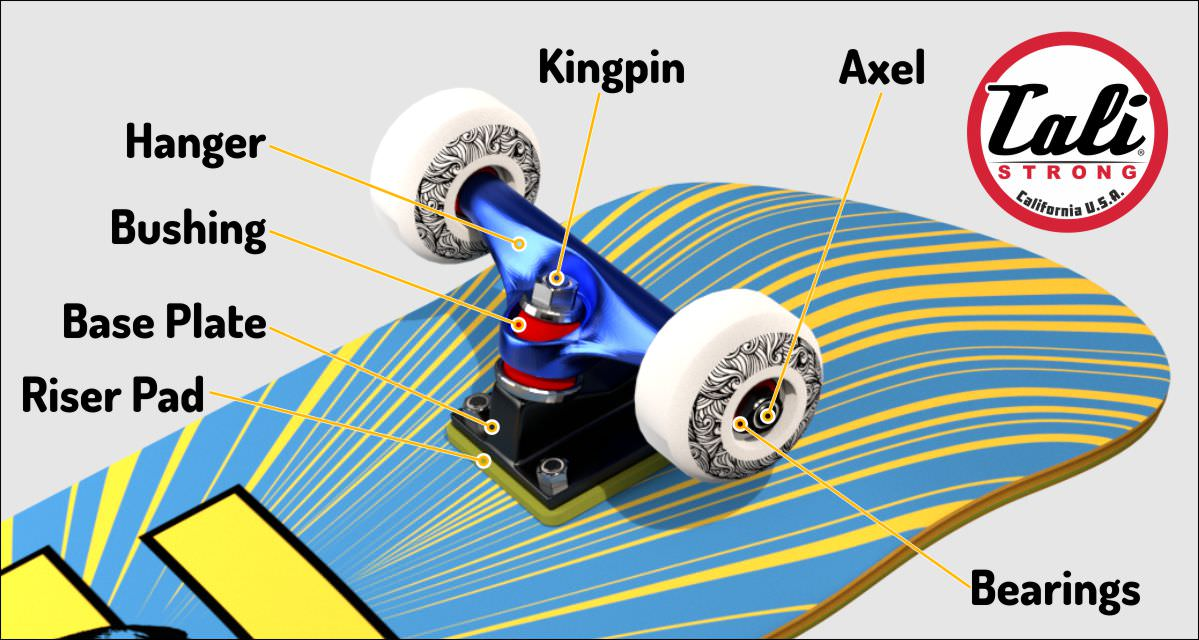
\includegraphics[width=.8\textwidth]{parts1.jpg}
\captionof{figure}{Skateboard Parts}
\label{parts1}
\end{minipage}%
\begin{minipage}{.5\textwidth}\centering
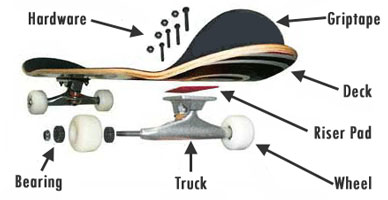
\includegraphics[width=.8\textwidth]{parts2.jpg}
\captionof{figure}{Skateboard Parts}
\label{parts2}
\end{minipage}
\end{figure}

\begin{itemize}
\item Deck - The surface on which the rider stands and to which the trucks and griptape are attached. It is essential for any deck to be sturdy, but also have some amount of flex for comfort. Decks vary in size and material, but they are typically wooden and a few feet long.
\begin{itemize}
\item Griptape - An adhesive surface for the top of the deck. One side is a very strong tape; the other side is a rough, sandpaper-like surface designed for high friction with the soles of the rider's shoes. Griptape comes in different grits (measure of “roughness”) and colors, but it is most often black.
\item Nose - Front of the board. A typical skateboard has a nose that is angled up.
\item Tail - Rear of the board. A typical skateboard has a tail that is angled up.
\end{itemize}
\item Trucks - The assemblies that connect the wheels to the deck. 
\begin{itemize}
\item Hanger - The main, T-shaped portion of the truck.
\item Riser Pad - A pad used to add distance between the wheel and the deck. Often made of a material conducive to dampening vibration, such as rubber or cork.
\item Baseplate - The metal piece of the truck that is bolted to the deck. The rest of the truck sits on a threaded rod that extends downwards from the baseplate.
\item Bushings - Spacers between the kingpin, the hanger, and the base plate. Bushings can be replaced to adjust the force required to turn while riding; i.e., a bushing that is harder to compress will require the user to lean to a direction more in order to perform the same degree of turn as a softer to compress bushing. Often made of some sort of rubber polymer.
\item Kingpin - A nut, usually a locknut, used to cap the hanger and bushing assembly. It can be loosened and tightened to fine tune the hardness of its bushing.
\item Axel - The rod used to attach the wheels, typically integral to the hanger. Axel nuts hold screw onto the axel's threaded ends to hold the wheels in place.
\item Bearings - Assemblies that sit between the axels and wheels to ensure smooth rotation.
\item Wheels - Skateboard wheels, vary in size, shape, color, and material (though typically they are some type of relatively hard plastic), but most are interchangeable without changing any other parts. Size and material can have significant effects on shock absorption and the frictional forces between the wheels and the road; a new set of wheels can drastically change the way that a skateboard handles.
\end{itemize}
\item Hardware - All the nuts and bolts needed to attach the trucks to the deck.
\item Longboard - Type of skateboard more suited for traveling long distances. Longboard decks are elongated and often somewhat flexible or bouncy; longboard trucks are typically looser (i.e. requiring less force to turn).
\end{itemize}

\subsection{Electric Skateboards}
An electric skateboard (ESB) is a skateboard with one or more electric motors and drive trains attached to one or more wheels. The battery that powers the motor(s) is generally fixed to the bottom of the deck in a shroud that protects it and accompanying electronics from damage. The motor is often controlled with a handheld controller which may be wireless or wired. Alternatively, some ESBs include pressure or strain sensors in the deck and use the rider's balance to control the motor. ESBs are usually longboards, as they tend to provide smoother rides at the higher speeds often achieved with the electric motor.\\
One example of a relatively standard ESB is the Boosted Board brand “Dual+ XR” pictured in figure \ref{boosted}, which happens to also be one of the most popular off the shelf ESBs on the market today.
\begin{figure}[!htbp]\centering
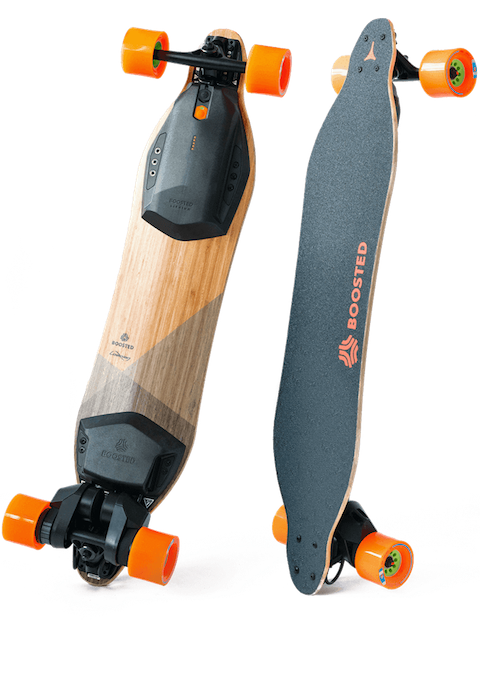
\includegraphics[width=.3\textwidth]{boosted.png}
\caption{Boosted Board Dual+ XR}
\label{boosted}
\end{figure}
It retails for \$1,599 and claims a top speed of 22 mph and a range of 14 miles with its 2000W motor and regenerative braking. Some more examples of popular ESBs can be found in table \ref{esbs}.
\begin{table}[!htbp]
\caption{Popular ESBs on the Market}
\label{esbs}
\resizebox{\textwidth}{!}{
\begin{tabular}{>{\bfseries}l l l l l}
\toprule
Board Name & Top Speed (mph) & Battery Range (miles) & Weight (lbs) & Price (Dollars) \\\hline
Inboard M1 & 22 & 7 & 14.5 & 1,000 \\
Boosted Plus/Stealth & 22/24 & 14 & 17 & 1,399/1.599 \\
Blink Qu4tro & 23 & 22 & 24 & 1,699 \\
Boosted Mini S/X & 18/20 & 7/14 & 15/16.8 & 749/999 \\
Onewheel +/+XR & 19 & 5-7/12-18 & 25 & 1,399/1,799 \\
\bottomrule
\end{tabular}
}
\end{table}

\section{System Overview} 
The modular electric skateboard is an electric skateboard with a deck comprised of multiple sections which can be interchanged and replaced, a handheld remote controller for controlling the electric motor, a rail/data bus system attached to the underside of the deck which is capable of housing a number of accessories, and a small computer system which manages those accessories via a simple but flexible API.

\subsection{Mechanical Systems}
\subsection{Control Systems and Control Processing}
Figure \ref{ctrl-overview} outlines the general structure of the motor control system.

%\includesvg[width=\textwidth]{rt}
%\input{figs/rt.pdf_tex}
\begin{figure}[!htbp]\centering
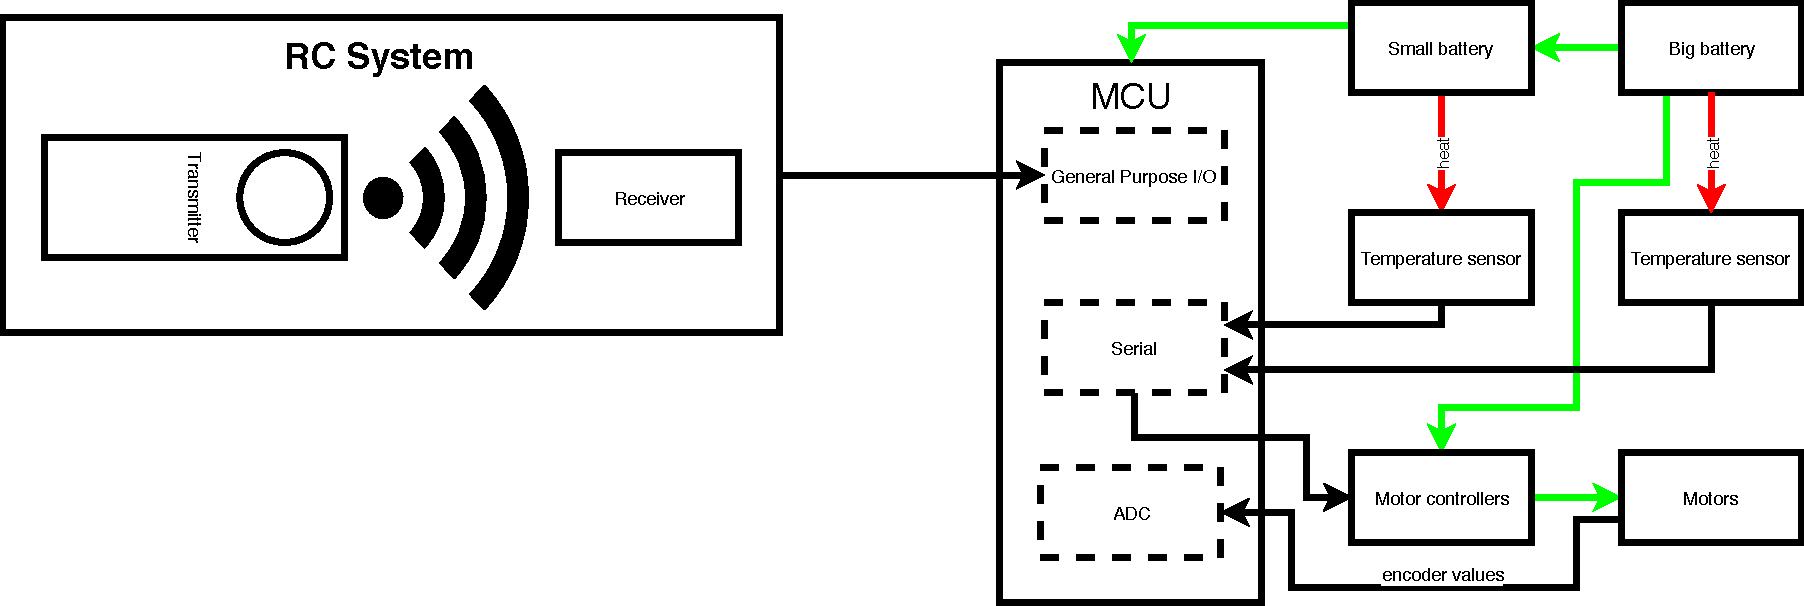
\includegraphics[width=\linewidth]{rt.pdf}
\caption{Major Components of Motor Control System}
\label{ctrl-overview}
\end{figure}
The remote control (RC) system is a standard 2.4 GHz hobbyist system designed for small unmanned RC cars and boats and comprised of a handheld transmitter, pictured in figure \ref{ctrl-tx}, and a small receiver which is attached to the vehicle being controlled. 
\begin{figure}[!htbp]\centering
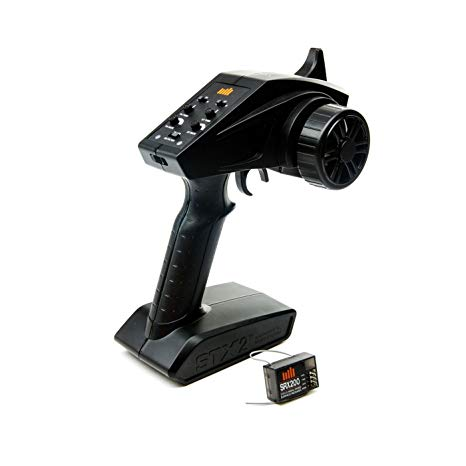
\includegraphics[width=0.5\textwidth]{controller.jpg}
\caption{Standard RC Transmitter and Receiver}
\label{ctrl-tx}
\end{figure}
The RC receiver outputs a pulse position modulation (PPM) signal that encodes the position of the throttle on the transmitter. This signal is read by the microcontroller (MCU). The MCU uses a PID control loop with throttle values, the temperatures of the primary and secondary batteries, and motor encoder readings as its inputs to determine the speed at which to drive the motors. The MCU software is structured as shown in figure \ref{mcu-sw}.
\begin{figure}[!htbp]\centering
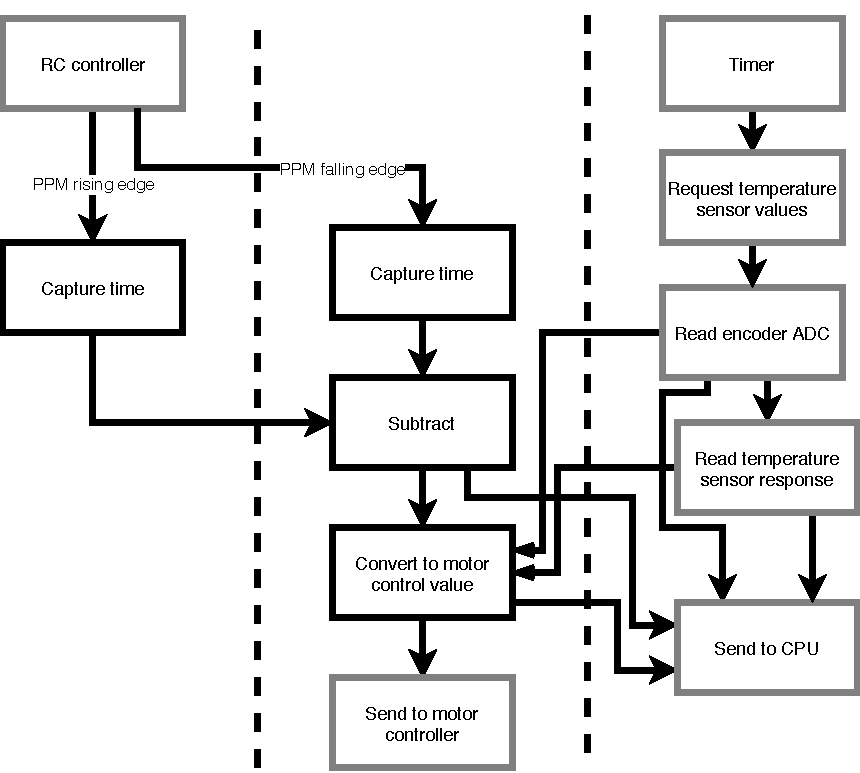
\includegraphics{mcusoftware.pdf}
\caption{Microcontroller Software Overview}
\label{mcu-sw}
\end{figure}

Each column represents a subroutine called by a hardware interrupt. In the case of the first two subroutines, the interrupt is triggered by the rising and falling edge, respectively of the PPM signal. On  the rising edge, a timer's value is captured. On the falling edge, the timer's value is captured again, and the difference between the times is the pulse position in which the throttle value is encoded. On each falling edge, an updated motor control value is decided based on the throttle position and based on encoder and temperature sensor values collected by a third interrupt routine and stored in global memory. The third routine is triggered at regular time intervals and collects temperature sensor and encoder values and sends them over a serial connection to the secondary computer system for long term storage.
\subsection{Electrical and Power Systems}
\subsubsection{Low Voltage Power}
The low voltage power system powers the MSP430 microcontroller, the Rock64 mini-PC, and any electronic accessories. Its main components are a battery comprised of two lithium cells for a total voltage of about 7.4 volts and a custom high-current voltage regulator that regulates to 5V. This regulator provides sufficient power to the MSP430 and Rock64, and can provide up to 2A at 5V to each accessory. For more information, see \ref{power-lv-sec}
\subsection{Computer and Accessory System}
Accessories are held in the dust resistant, water resistant (IP 66, see section \ref{} for more details shrouds mounted to the underside of the deck, which also contain other electronic systems. Figure \ref{access-full} shows the shrounds mounted on the deck, while figure \ref{access-expl} shows an exploded view of the shroud itself.
\begin{figure}
  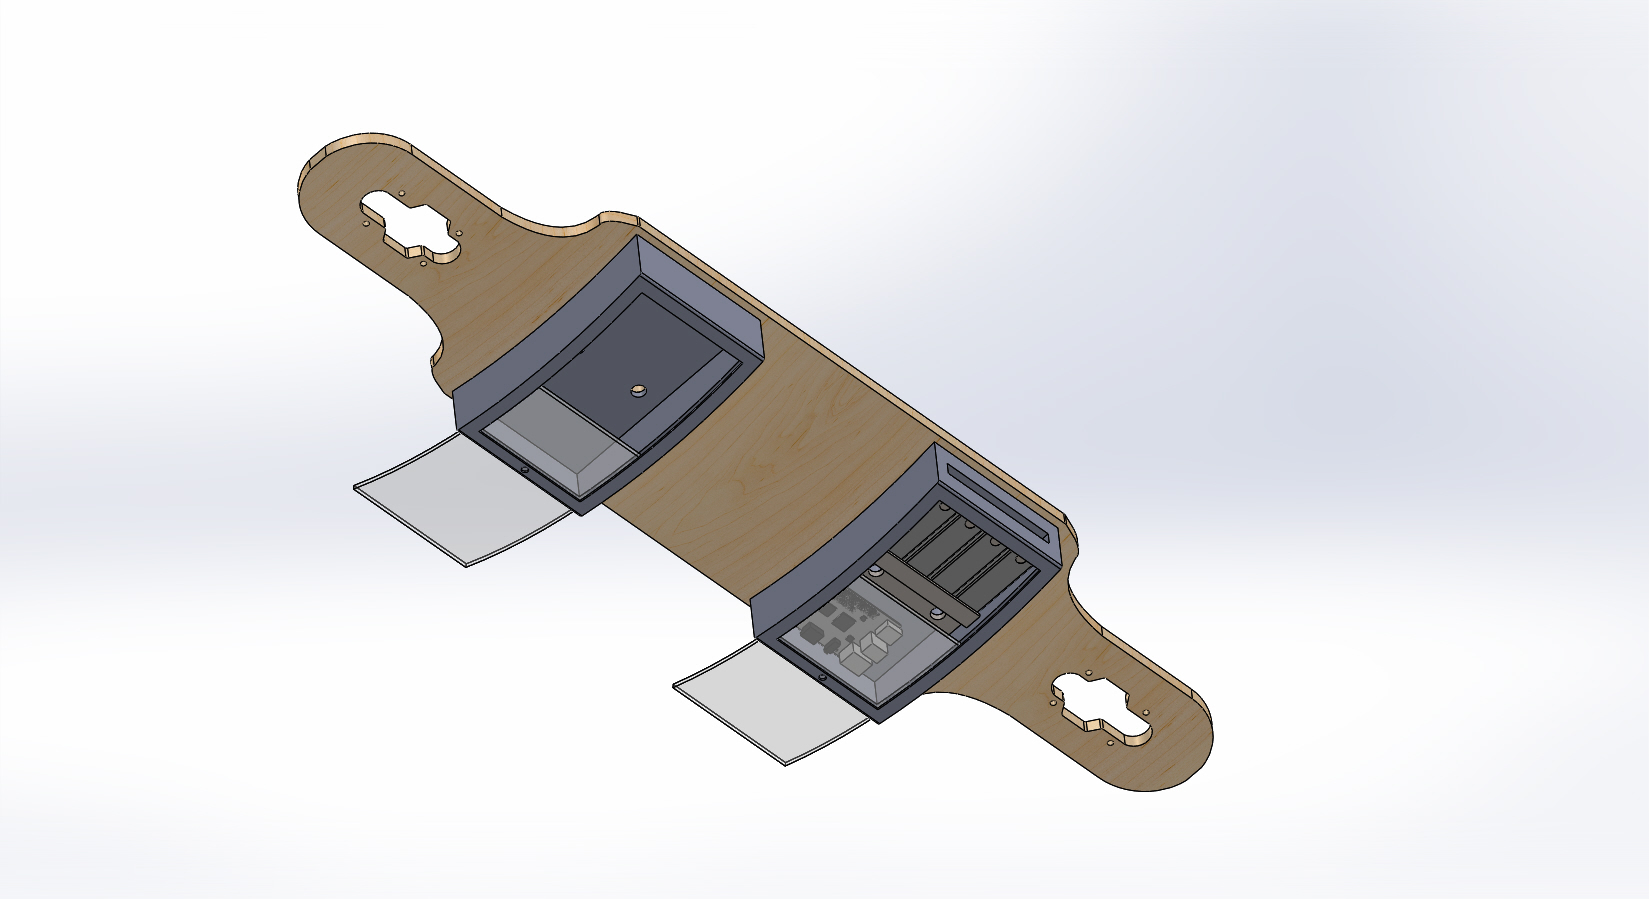
\includegraphics{ModularAssembledBottomAngle}
  \caption{Electronics Shrouds}
  \ref{access-full}
\end{figure}
\begin{figure}
  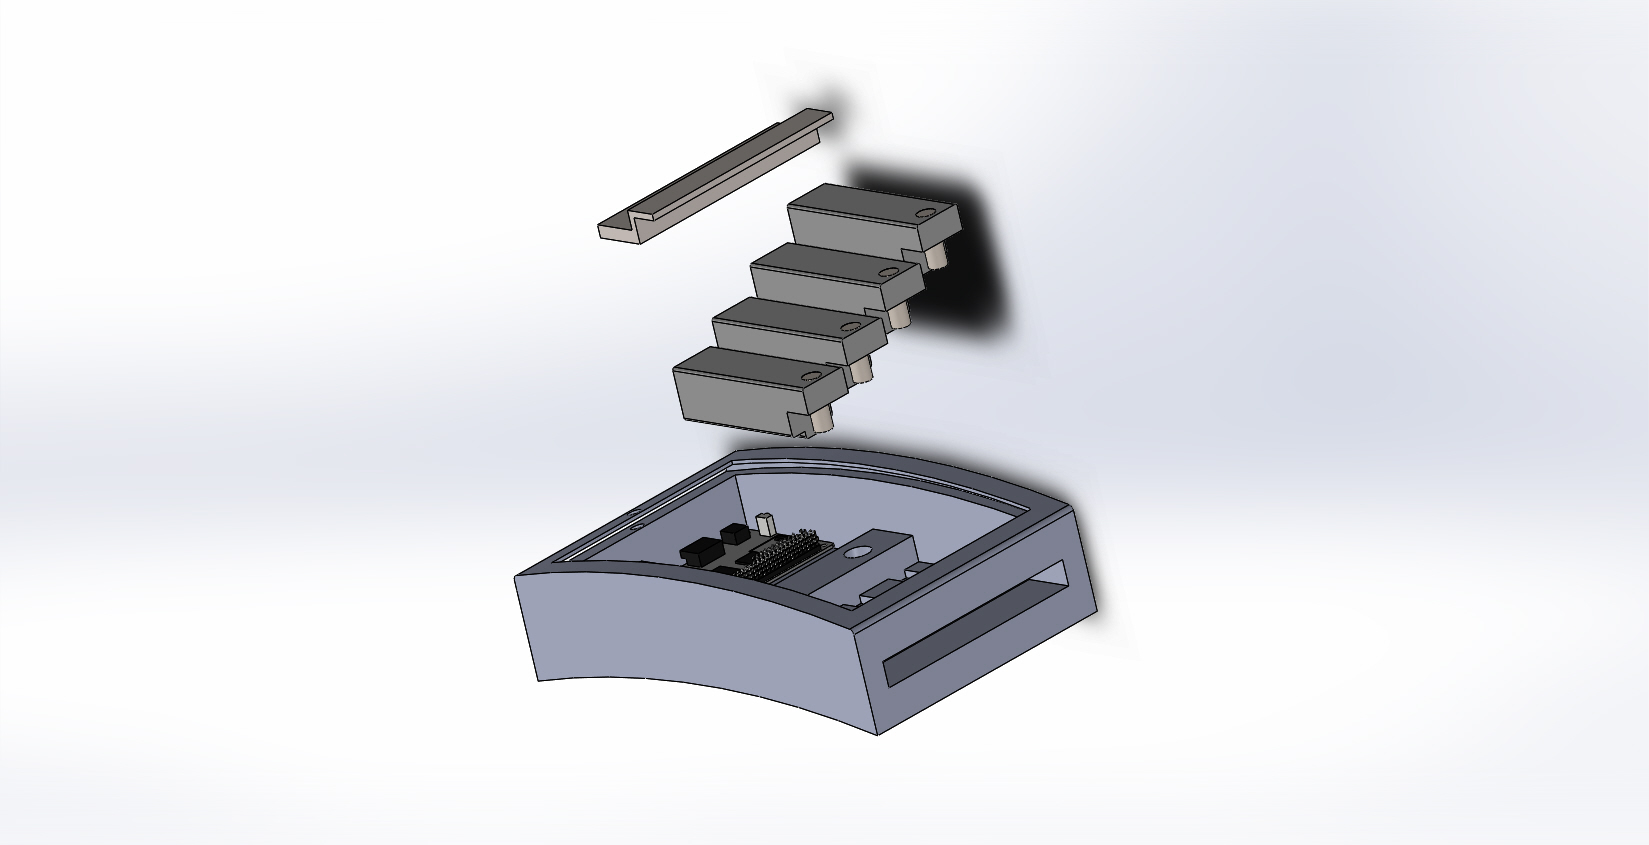
\includegraphics{ModPieceAngleExtend}
  \caption{Exploded View of Accessory System in Shroud}
  \ref{access-expl}
\end{figure}
Accessories slot into the base of the shroud, and then the horizontal beam is bolted on top of them to secure them during use. On the end opposite the beam is the accessory's Mini-DIN plug (for more detail, see \ref{access-plug}), used for power and data, which plugs into a port mounted to a PCB mounted to the shroud.

\section{Design Analysis}
\subsection{Trade Studies}
This section breaks down in detail several tradeoffs of components, protocols, etc. which had to be considered once the system level design was finished. Each column compares the qualities of a certain attribute of the systems under study, and lists the point value score assigned to each quality. The maximum acheivable score in each category is listed in the header of each category with a ``/'' preceding it; the maximum acheivable total score is listed in the header of the leftmost column listing the names of the systems being compared.

\subsubsection{Real Time Microcontroller}
Before choosing a specific processor or development board, several microcontroller (MCU) platforms were compared. At least some variants of each of the microcontrollers in table \ref{tr-mcu} would meet the basic requirements of the MCU for the real time control system on the MESB, such as hardware interrupts and an appropriate number of analog to digital converters, timers, etc.
\begin{table}[!htbp]
\caption{Real Time Microcontroller Trade Study}
\label{tr-mcu}
\resizebox{\textwidth}{!}{
\begin{tabular}{>{\bfseries}l>{\bfseries}r lr lr lr lr lr}
\toprule
%platform & Total Points & Price & Points (5) & architecture & Points (4) & clock & Points (2) & current draw & Points (2) & Familiarity/ease of use & Points (6)
%\tradecat{Platform} & \tradecat{Price} \\
\thead{Platform} & /20 & \thead{Price} & /5 & \thead{Architecture} & /5 & \thead{Core \\ Clock} & /2 & \thead{Current \\ Draw } & /2 & \thead{Familiarity \\ \& Ease of Use} & /6\\
\cmidrule(r){1-2} \cmidrule(r){3-4} \cmidrule(r){5-6} \cmidrule(r){7-8} \cmidrule(r){9-10} \cmidrule(r){11-12}
%Name & Total Points & Price & Points\\
MSP430 & 16 & \$10-18 & 4 & 16 bit RISC & 3 & 8-24 MHz & 1 & ~5 mA & 2 & High & 6\\
STM32 Cortex & 13 & \$10-25 & 4 & 32 bit ARM Cortex-m & 4 & 32-400MHz & 2 & ~100-500 uA/MHz & 0 & Moderate & 3\\
ATMega328P & 15 & \$3-10 & 5 & 8 bit AVR RISC & 1 & up to 20 MHz & 1 & ~5 mA & 2 & High & 6\\
\bottomrule
\end{tabular}
}
\end{table}
Though all of these platforms had their advantages and disadvantages, the MSP430 was chosen for its capable and flexible 16-bit architecture, its low cost and power consumption, and for the developers' familiarity with the ins and outs of its hardware and firmware.

Table \ref{tr-msp} compares various MSP430 development boards. The names are truncated to avoid redundancy and save space; the development boards being compared are the MSP-EXP430FR2355, MSP-EXP430FR2433, etc., using the MSP430FR2355, MSP430FR2433, etc. microprocessors, respectively.\\
\begin{table}[!htbp]
\caption{MSP430 Trade Study}
\label{tr-msp}
\resizebox{\textwidth}{!}{
\begin{tabular}{>{\bfseries}l>{\bfseries}r lr lr lr lr lr}
\toprule
\thead{MCU} & /15 & \thead{Price}& /8 & \thead{Core Clock} & /2 & \thead{RAM + \\ Storage} & /5 & \thead{Current Draw} & /3 & \thead{ADCs} & /2 \\
\cmidrule(r){1-2} \cmidrule(r){3-4} \cmidrule(r){5-6} \cmidrule(r){7-8} \cmidrule(r){9-10} \cmidrule(r){11-12}
FR2355 & 12 & \$13 & 5 & 24 MHz & 2 & 32KB & 2 & 142 uA/MHz,{\raise.5ex\hbox{$\scriptstyle\sim$}}1 uA standby & 1 & 1x12b & 2\\
FR2433 & 13 & \$10 & 8 & 16 MHz & 1 & 15.5KB & 1 & 125 uA/MHz; $<$1 uA standby & 2 &8x10b & 1\\
FR5994 & 11 & \$17 & 1 & 16 MHz & 1 & 264KB & 5 & 118 uA/MHz; 500 nA standby & 2 & 1x12b & 2\\
FR4133 & 10 & \$14 & 4 & 16 MHz & 1 & 15.5KB & 2 & 126 uA/MHz; $<$1 uA standby & 2 &10x10b &1\\
FR6989 & 10 & \$18 & 0 & 16 MHz & 1 & 128KB & 4 & 100 uA/MHz; 350 nA standby & 3 & 16x12b & 2\\
FR5969 & 11 & \$16 & 2 & 16 MHz & 1 & 62KB & 3 & 100 uA/MHz; .4 uA standby & 3 & 16x12b & 2\\
F5529 & 16 & \$13 & 5 & 25 MHz & 2 & 136KB & 4 & 150 uA/MHz; 2 uA standby & 3 & 1x12b & 2\\
\bottomrule
\end{tabular}
}
\end{table}
The MSP430F5529 offers above average MSP430 performance for below average price. While its higher clock rate may not be necessary, 128KB of flash memory provide a comfortable amount of program storage space
\subsubsection{Accessory Bus Serial Protocol}
Table \ref{tr-serial} compares several serial protocols which were considered for the main accessory bus:
\begin{table}[!htbp]
\caption{Accessory Bus Serial Protocol Trade Study}
\label{tr-serial}
\resizebox{\textwidth}{!}{
\begin{tabular}{>{\bfseries}l>{\bfseries}r lr lr lr lr }
\toprule
\thead{Name} & /27 & \thead{Wires, \\ Shared} & /3 & \thead{Add'l Wires \\ per Device }& /10 & \thead{Speed} & /4 & \thead{Ease\\ of Use} & /10\\
\cmidrule(r){1-2} \cmidrule(r){3-4} \cmidrule(r){5-6} \cmidrule(r){7-8} \cmidrule(r){9-10} 
\itwoc & 25 & 2 & 2 & 0 & 10 & 100k-3.4Mbps & 3 & easy & 10\\
CAN & 17 & 2 & 2 & 0 & 10 & 1Mbps & 3 & hard & 2\\
SPI & 15 & 3 & 1 & 1 & 3 & 10Mbps & 4 & medium & 7\\
UART & 15 & 0 & 3 & 2 & 0 & {\raise.5ex\hbox{$\scriptstyle\sim$}}10-100kbps & 2 & easy  & 10\\
LIN & 17 & 1 & 3 & 0 & 10 & 20kbps & 1 & hard & 3\\
\bottomrule
\end{tabular}
}
\end{table}
\itwoc{} was chosen for its two-wire communication, ease of use, and more than sufficient speed. Some other serial protocols shared some but not all of these desirable attributes, but \itwoc{} scored nearly perfectly overall.

\subsubsection{Data Connector Plug and Socket}
Table \ref{tr-conn} compares several types of connectors which were considered for the data/power connections to accessories:
\begin{table}[!htbp]
\caption{Data Connector Trade Study}
\label{tr-conn}
\resizebox{\textwidth}{!}{
\begin{tabular}{>{\bfseries}l>{\bfseries}r lr lr lr lr lr lr lr lr lr }
\toprule
\thead{Name} & /21 & \thead{Data\\Lines} & /2 & \thead{Water\\Resistance} & /2 & \thead{Locking} & /2 & \thead{Terminal\\Area} & /3 & \thead{Terminal\\Length} & /3 & \thead{Price/\\Pair} & /3 & \thead{Strength} & /2 & \thead{Current\\(A)} & /2 & \thead{Voltage\\(V)} & /2\\
\cmidrule(r){1-2} \cmidrule(r){3-4} \cmidrule(r){5-6} \cmidrule(r){7-8} \cmidrule(r){9-10} \cmidrule(r){11-12} \cmidrule(r){13-14} \cmidrule(r){15-16} \cmidrule(r){17-18} \cmidrule(r){19-20}
TRRS 3.5mm & 15 & 2 & 2 & No & 1 & No & 1 & Small & 3 & Small & 3 & \$2-5 & 2 & Yes & 2 & 1 & 1 & 5 & 1 \\
Mini-DIN & 19 & 1-7 & 2 & Yes & 2 & No & 1 & Small & 3 & Small & 3 & \$2-5 & 2 & Yes & 2 & 2-7 & 2 & 30 & 2\\
Micro USB-B & 11 & 3 & 2 & Yes & 2 & No & 1 & Small & 3 & Small & 3 & \$3-7 & 1 & No & 1 & 2 & 2 & 5 & 1 \\
Mini USB-B & 19 & 3 & 2 & Yes & 2 & No & 1 & Small & 3 & Small & 3 & \$1 & 3 & Yes & 2 & 1 & 1 & 2-5 & 1 \\
4P4C & 18 & 2 & 2 &  Yes (IP67) & 2 & Yes & 2 & Small & 3 & Small & 3 & \$1 & 3 & Yes & 2 & 1 & 1 & 2-5 & 1 \\
8P8C & 19 & 6 & 2 &  Yes (IP67) & 2 & Yes & 2 & Small & 3 & Small & 3 & \$1 & 3 & Yes & 2 & 2 & 2 & 2-5 & 1 \\
DE-9 & 18 & 7 & 2 &  Yes & 2 & Yes & 2 & Large & 1 & Medium & 2 & \$1-2 & 2 & Yes & 2 & 5 & 2 & 100 & 2\\
\end{tabular}}
\end{table}

\subsubsection{Low Voltage Power}\label{power-lv-sec}
A potential low voltage power system, for the microcontroller, CPU, and accessories, was designed in OrCAD Capture for simulation in PSpice. Figure \ref{power-lv} shows the circuit. 
\begin{figure}[!htbp]
  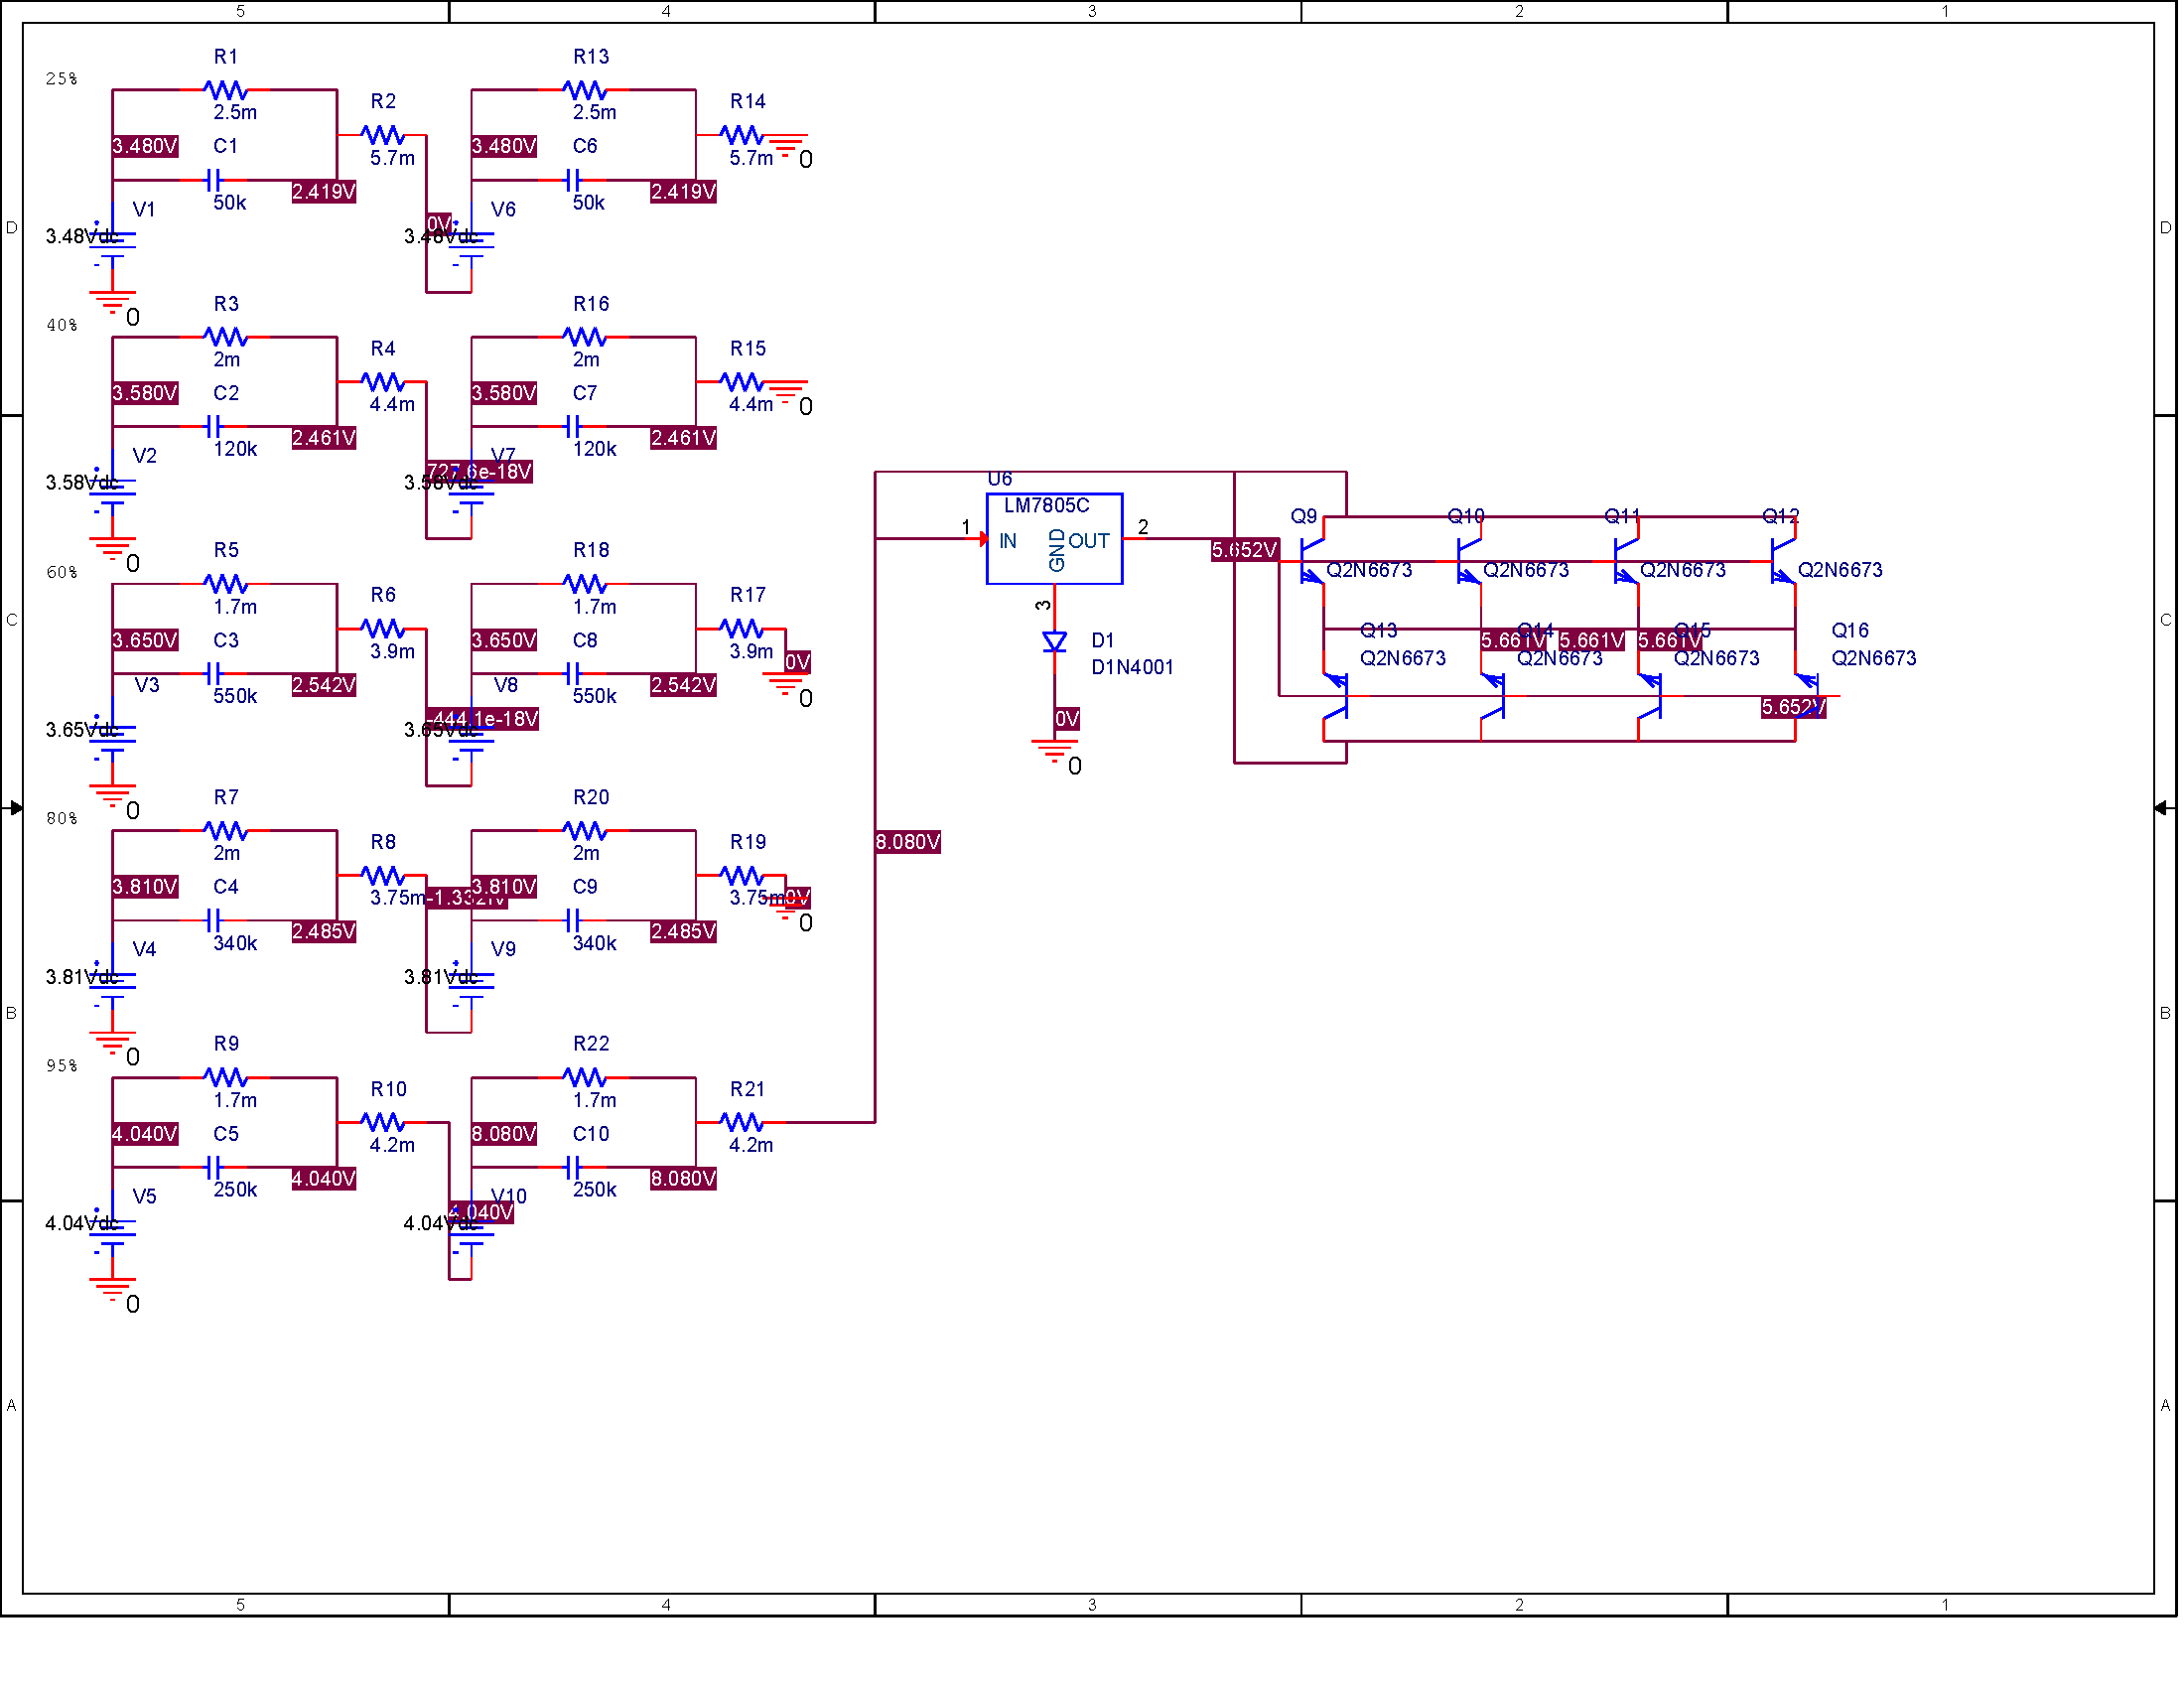
\includegraphics{power.xps.pdf}
  \caption{Low Voltage Power Circuit Schematic}
  \label{power-lv}
\end{figure}
There was no PSpice model available for the battery, so a model using experimentally determined voltages, resistances, and capicatances was implemented. The left hand side of the circuit is an array of different battery models for the same lithium cell at different charges, which are show on the top left. Pairs of identical models are connected in series because the circuit requires two lithium cells. The right hand side is the regulator circuit, composed of a simple LM7805 5V voltage regulator and several bypass power transistors to drive additional current. To ensure that the regulator circuit can provide steady voltage and that the batteries will stay within safe operating boundaries, the sets of batteries will be connected one at a time to the regulator circuit, and the regulator circuit will be connected to a load. Transient and steady-state characteristics of battery and regulator current and voltage will be measured to ensure safe and reliable operation.
\end{document}
